\documentclass{template}
\usepackage{array}
\usepackage[ngerman]{babel}
\usepackage{graphicx}


\SetTitle{\textbf{Proposal für die Bachelorarbeit}\\
Intersektionales Wohlbefinden im Stadtraum: Entwicklung und Test einer App}
\SetAuthor{Lukas Batschelet, \href{mailto:lukas.batschelet@students.unibe.ch}{lukas.batschelet@students.unibe.ch} \\ 
Betreuung: Moritz Gubler \textit{(+ Carolin Schurr)}}
\SetDate{\today}

\AddBibFile{references.bib}




\begin{document}
\maketitle

\section{Problemstellung \& Motivation}
Das Wohlbefinden im urbanen Raum hängt sowohl von räumlichen Faktoren (z.\,B.\ Infrastruktur, Grünflächen) als auch von sozialen Aspekten (z.\,B.\ Ungleichheit, Sicherheitsgefühl) ab. Studien zeigen einen engen Zusammenhang zwischen Umgebungseinflüssen und psychischer Gesundheit bzw.\ subjektivem Wohlbefinden \parencite{kan_impacts_2022, hammoud_smartphone-based_2024, bergou_mental_2022}. Zugleich verdeutlichen \textbf{intersektionale Ungleichheiten} – Überschneidungen von Geschlecht, Herkunft und sozioökonomischem Status – die Bedeutung sozialer Kategorien für die Wahrnehmung und Nutzung des Stadtraums \parencite{webster_centering_2021, rodo-de-zarate_developing_2014, beebeejaun_race_2022}.

Einige digitale Werkzeuge greifen diese Themen bereits auf. \emph{Urban Mind} \parencite{bakolis_urban_2018} erhebt wiederholt ortsbezogene Daten zum mentalen Wohlbefinden, verzichtet jedoch auf einen intersektionalen Fokus. \emph{InterMaps} \parencite{rodo-de-zarate_developing_2014} integriert Intersektionalität und Raum, basiert aber auf einer einmaligen, retrospektiven Erhebung ohne laufende Geolokalisierung. Beide sind nicht quelloffen. Eine Anwendung, die wiederholte Erhebungen \emph{und} intersektionale Kategorien kombiniert, liegt bislang nicht vor.

Diese Bachelorarbeit soll daher eine \textbf{mobile App} entwickeln, welche Stärken beider Tools verbindet und methodische Lücken schliesst. Durch regelmässige, ortsbezogene Befragungen, die verschiedene soziale Kategorien berücksichtigen, werden \emph{alltägliche} und intersektionale Daten zum Wohlbefinden erhoben. Zugleich möchte ich meine persönliche Motivation, ein Softwareprojekt umzusetzen, einbringen und eine Anwendung schaffen, die offen genutzt und weiterentwickelt werden kann.



\section{Zielsetzung \& Fragestellungen}
Das Ziel dieser Arbeit ist die Entwicklung und Erprobung einer mobilen App, die intersektionales Wohlbefinden im Stadtraum in Echtzeit erfassen kann. Die App soll es ermöglichen, ortsbezogene Daten über subjektives Wohlbefinden unter Berücksichtigung intersektionaler Kategorien zu sammeln.

Die zentrale Forschungsfrage lautet:
\begin{itemize}
    \item \emph{Wie kann intersektionales Wohlbefinden im Stadtraum mit einer digitalen Anwendung erfasst werden?}
\end{itemize}

Weitere Unterfragen sind:
\begin{itemize}
    \item Welche methodischen und technischen Anforderungen muss eine solche App erfüllen?
    \item Wie müssen Fragen zur Erfassung von intersektionalem Wohlbefinden formuliert sein?
    \item Welche Herausforderungen ergeben sich bei der Entwicklung und Testung der App?
\end{itemize}

\section{Methodisches Design}
\subsection{Technische Umsetzung}
Die App wird mit \textbf{React Native (Expo)} \footnote{\href{https://expo.dev/}{https://expo.dev/}} als Frontend-Technologie und \textbf{Supabase}\footnote{\href{https://supabase.com/}{https://supabase.com/}} als Backend-Datenbank umgesetzt. Dies ermöglicht eine plattformübergreifende Entwicklung und eine sichere und flexible Datenverwaltung.

Mögliche Funktionen sind:
\begin{itemize}
    \item \textbf{Geolokalisierte Fragen}: Automatische Erfassung des Aufenthaltsorts
    \item \textbf{Tägliche Erinnerungen}: Drei kurze Erhebungen pro Tag
    \item \textbf{Intersektionale Kategorien}: Nutzer*innen geben einmalig demografische Informationen an
\end{itemize}

\subsubsection{Datenschutz.}
Da die App \textbf{sensible Daten} zum Wohlbefinden und zum Standort erfasst, stehen datenschutzrechtliche Überlegungen an oberster Stelle. Folgende Prinzipien sollen sicherstellen, dass die Datenerhebung möglichst risikoarm erfolgt:

\begin{itemize}
    \item \textbf{Pseudonymisierung}: Die Teilnehmenden werden nur über eine zufällig generierte ID erfasst. Es werden keine Namen, E-Mail-Adressen oder anderen direkt zuordenbaren Identifikatoren gespeichert.
    \item \textbf{Minimaler Datensatz}: Altersangaben erfolgen nur in groben Kategorien (z.\,B.\ 18–25, 26–35 usw.), Standortdaten werden nur in einer geringen Genauigkeit erfasst (z.\,B.\ +/- 200 Meter).
    \item \textbf{Datenspeicherung \& Löschung}: Die Daten werden auf einer Cloud-Plattform mit den entsprechenden Zugriffsrechten gespeichert. Proband*innen haben jederzeit das Recht, ihre Daten vollständig zu löschen.
    \item \textbf{Open-Source-Entwicklung}: Der Quellcode der App wird offen zugänglich sein, sodass Datenschutzvorkehrungen transparent dargelegt und überprüft werden können.
\end{itemize}

Durch diese Massnahmen folgt das Projekt den Grundsätzen \textit{Privacy by Design} und \textit{Privacy by Default}.

\subsection{Fragebogenentwicklung, Datenerhebung und Pilotphase}

Ein zentraler Schritt dieser Arbeit ist die Entwicklung eines Fragebogens zur Erfassung intersektionalen Wohlbefindens im Stadtraum. Um bewährte Methoden einzubinden, wird auf bestehende Skalen zur Messung von Wohlbefinden (z.\,B.\ WHO-5, SWEMWBS, PANAS) zurückgegriffen. Diese werden durch zusätzliche Items ergänzt, die verschiedene Dimensionen von Intersektionalität berücksichtigen. Da keine standardisierten Skalen existieren, welche Intersektionalität direkt messen, erfolgt dies über eine Kombination aus soziodemografischen Angaben (in möglichst groben Kategorien) und Fragen zur subjektiven Wahrnehmung bestimmter Orte und Situationen. Die Arbeit von Maria Rodó-de-Zárate \textcite{rodo-de-zarate_developing_2014} bietet dafür relevante theoretische und methodische Anknüpfungspunkte.

\subsubsection{Pilotphase.}
Da diese Bachelorarbeit nur einen begrenzten zeitlichen Rahmen abdeckt, ist keine gross angelegte Studie vorgesehen. Stattdessen wird eine \textit{kurze Pilotphase} (voraussichtlich mit 5–10 Teilnehmenden) durchgeführt, um die grundlegende Funktionsfähigkeit der App und die Akzeptanz der Befragungen zu testen. Diese Pilotphase dient dazu, erste explorative Erkenntnisse über die Nutzbarkeit der Daten zu gewinnen. Folgende Ziele stehen im Vordergrund:

\begin{itemize}
    \item \textbf{Technische Validierung}: Überprüfung, ob die App stabil läuft und die Standorterfassung zuverlässig funktioniert.
    \item \textbf{Benutzerfreundlichkeit}: Einsammeln von Feedback zum Fragebogen (Verständlichkeit, Länge, Relevanz) und zur Bedienoberfläche.
    \item \textbf{Datenauswertung im Kleinen}: Erste Auswertungen der erhobenen Daten, um festzustellen, ob sich Muster erkennen lassen, wie Teilnehmende ihr Wohlbefinden in Abhängigkeit von Ort und Situation einschätzen.
\end{itemize}

Eine umfassende statistische Auswertung oder repräsentative Aussagen zum intersektionalen Wohlbefinden sind in diesem Umfang \textit{nicht} realistisch. Die Erkenntnisse aus der Pilotphase können jedoch wertvolle Hinweise darauf liefern, inwieweit eine grössere Studie sinnvoll wäre. Eine solche Folgestudie könnte beispielsweise im Rahmen einer künftigen Masterarbeit oder eines anderen Forschungsprojekts durchgeführt werden.





\section{Zeitplan}

\begin{figure}[h]
    \centering
    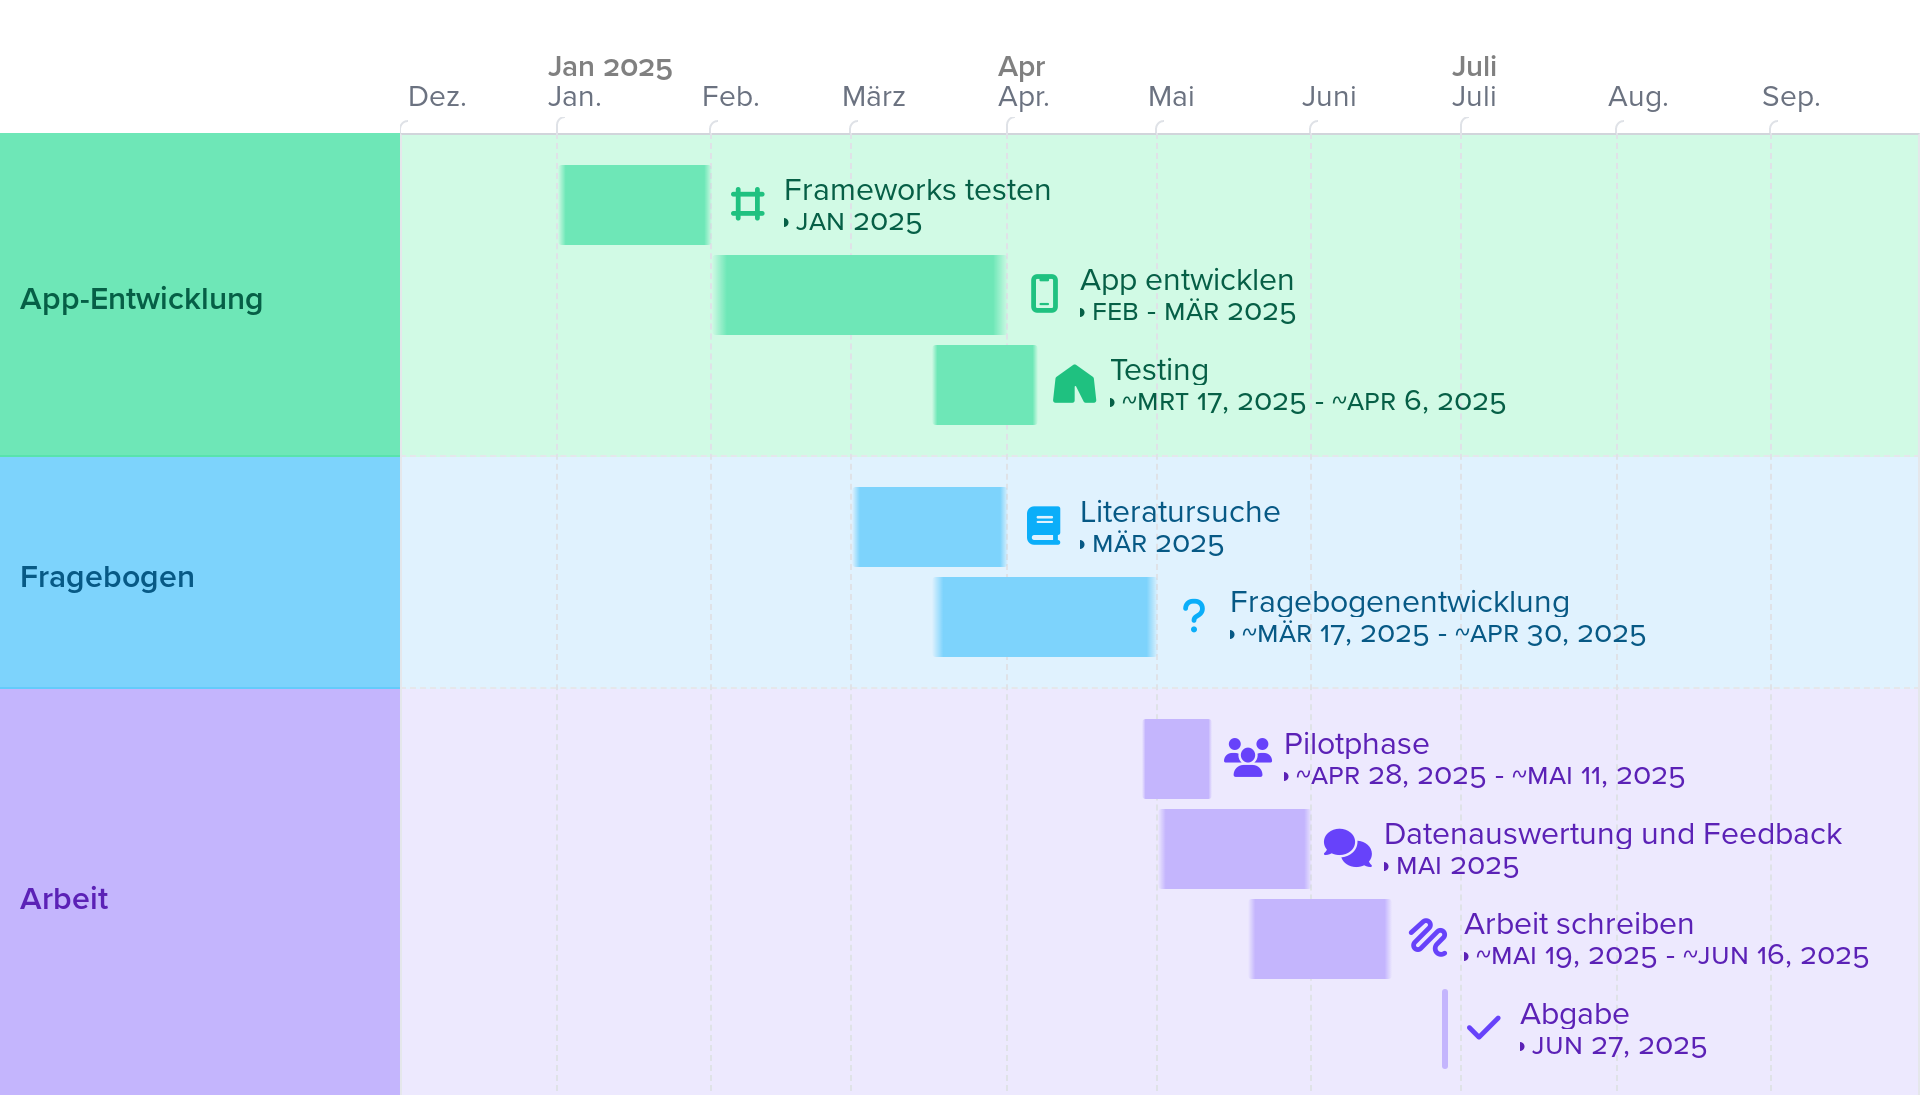
\includegraphics[width=1\linewidth]{timeline_proposal.png}
\end{figure}


\section{Erwarteter Beitrag der Arbeit}
Diese Bachelorarbeit verbindet geographische Forschung mit technischen Entwicklungen und leistet einen Beitrag zur Methodik der intersektionalen Stadtforschung. Die erstellte App kann als Open-Source-Tool weiterentwickelt und für zukünftige Forschungsprojekte genutzt werden.

% ----------------- Bibliographie ------------------
\newpage
\PrintBib

\section*{Hinweis für den Einsatz von künstlicher Intelligenz (KI)}

Dieses Dokument wurde mit Hilfe von KI-basierten Tools überarbeitet. LanguageTool, ein KI-gestütztes Grammatik- und Stilprüfungswerkzeug, wurde verwendet, um Formulierungen zu verbessern und die Grammatik zu korrigieren. Chat-GPT von Open-AI wurde verwendet, um Feedback zur Klarheit und Strukturierung des Textes zu erhalten. Es wurde keine KI zur Erstellung von Originalinhalten verwendet.

\end{document}
